\section{U-Net}
2015 yılında Olaf Ronneberger ve arkadaşları tarafından "U-Net: Convolutional Networks for Biomedical Image Segmentation" makalesinde duyurulmuştur. İsmindeki "U" harfi mimarisi U harfine benzemesinden gelmektedir. Az miktarda veri ile eğitilebilir. Contracting Path (Daraltıcı Yol) ve Expansive Path (Genişletici Yol) olmak üzere iki bölümden oluşur.

\begin{figure}[ht]
    \centering
    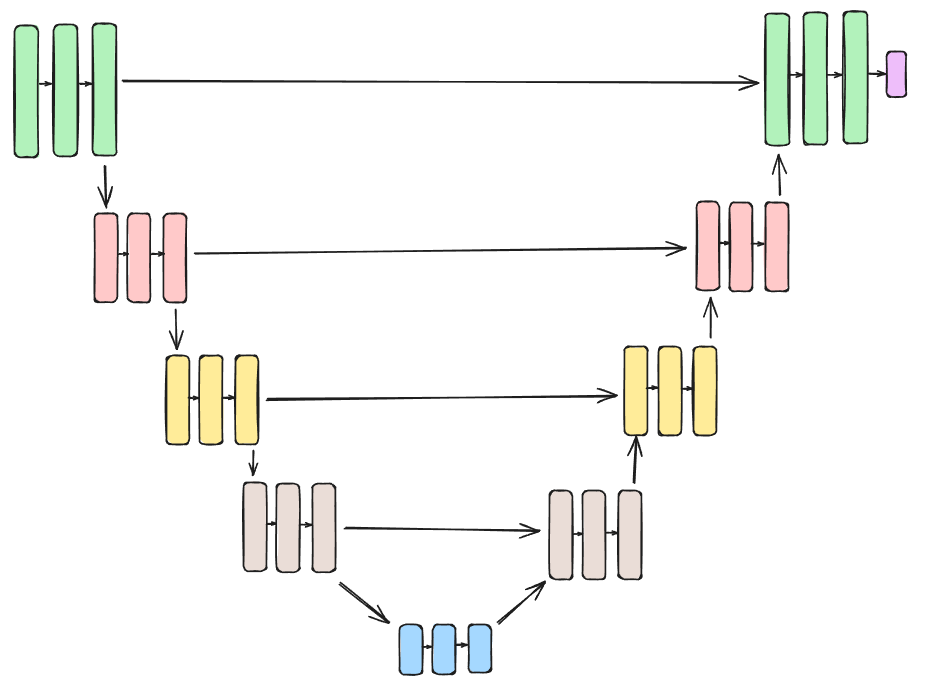
\includegraphics[width=0.8\textwidth]{images/unet_architecture.png}
    \caption{U-Net mimarisi.}
    \label{fig:enter-label}
\end{figure}

\begin{itemize}
    \item \textbf{Contracting Path (Daraltıcı Yol):} Giriş görüntüsünün boyutunu azaltan ve özellik haritaları oluşturan bir dizi konvolüsyon katmanı içerir. Her konvolüsyon katmanı ReLU aktivasyon fonksiyonu ve bir max pooling katmanı ile birleştirilir. Böylece görüntünün büyük ölçekli öznitelikleri daha küçük bir boyuta sıkıştırılır.
    \item \textbf{Expansive Path (Genişletici Yol):} Daraltıcı yolun çıktısını orijinal boyutlara geri dönüştüren bir dizi konvolüsyon ve upsampling (yukarı örnekleme) katmanı içerir. Her adımda, bir upsampling katmanı ve bir veya birden fazla konvolüsyon katmanı bulunur. Böylece, küçültülmüş özellik haritaları görüntünün orijinal boyutlarına genişletilir.
\end{itemize}

Encoder, görüntüyü daha küçük boyutlara ve daha fazla sayıda kanala dönüştürür. Decoder, kodlayıcı tarafından üretilen küçük boyutlu görüntüyü, orijnal görüntü boyutuna geri döndürür. U-Net asimetrik bir yapıya sahiptir. Encoder aşağı örnekleme (downsampling) katmanları eklerken, decoder yukarı örnekleme (upsampling) katmanları ekler. U-Net skip connections adındaki encoder katmanlarından decoder katmanlarına direkt bağlantılar ekleyen bir mimarı kullanır. Bu, daha yüksek seviyeli özelliklerin daha düşük seviyeli özelliklerle birleştirilmesini sağlar, böylece modelin hem lokal hem de global özellikleri öğrenmesini sağlar. 

\subsection{Python Kodu}

\begin{lstlisting}[language=Python]
import tensorflow as tf
from tensorflow.keras.layers import Conv2D, MaxPooling2D, Conv2DTranspose, Concatenate
from tensorflow.keras.models import Sequential

def conv_block(filters, kernel_size=(3, 3), activation='relu', padding='same'):
    return Sequential([
        Conv2D(filters, kernel_size, activation=activation, padding=padding),
        Conv2D(filters, kernel_size, activation=activation, padding=padding)
    ])

def unet_model(input_size=(256, 256, 3)):
    model = Sequential()
    
    # Encoder
    model.add(conv_block(64, input_shape=input_size))
    model.add(MaxPooling2D(pool_size=(2, 2)))
    
    model.add(conv_block(128))
    model.add(MaxPooling2D(pool_size=(2, 2)))
    
    model.add(conv_block(256))
    model.add(MaxPooling2D(pool_size=(2, 2)))
    
    model.add(conv_block(512))
    model.add(MaxPooling2D(pool_size=(2, 2)))
    
    # Middle
    model.add(conv_block(1024))
    
    # Decoder
    model.add(Conv2DTranspose(512, (2, 2), strides=(2, 2), padding='same'))
    model.add(Concatenate())
    model.add(conv_block(512))
    
    model.add(Conv2DTranspose(256, (2, 2), strides=(2, 2), padding='same'))
    model.add(Concatenate())
    model.add(conv_block(256))
    
    model.add(Conv2DTranspose(128, (2, 2), strides=(2, 2), padding='same'))
    model.add(Concatenate())
    model.add(conv_block(128))
    
    model.add(Conv2DTranspose(64, (2, 2), strides=(2, 2), padding='same'))
    model.add(Concatenate())
    model.add(conv_block(64))
    
    # Output
    model.add(Conv2D(1, (1, 1), activation='sigmoid'))
    
    return model

model = unet_model()
model.summary()
\end{lstlisting}

\subsection{Varyasyonları}
\begin{itemize}
    \item \textbf{V-Net:} U-Net'in 3D versiyonudur. Hacim verileri üzerinde segmentasyon yaparken daha fazla derinlik ve boyutluluğa izin verir.
    \item \textbf{Attention U-Net:} Attention mekanizması, U-Net'in her katmanına eklenir ve daha az önemil özellik haritalarının göz ardı edilmesini sağlar. Böylece daha önemli özellikler vurgulanır.
    \item \textbf{Residual U-Net:} U-Net'e skip connection'ların eklenmesiye daha fazla derinlik ve öğrenme kapasitesi kazandırmak için Residual Block'ları kullanır.
    \item \textbf{U-Net++:} U-Net'in kodlayıcı ve kod çözücü katmanlarına atlama bağlantıları ekleyen bir varyasyondur. Bu sayede, farklı seviyelerdeki özelliklerin daha iyi bir şekilde entegre edilmesi sağlanır.
    \item \textbf{ResUNet:} Kalıntı ağları (ResNet) ile U-Net mimarisini birleştiren bir varyasyondur.
\end{itemize}

\newpage